\documentclass[a4paper, 12pt, openany]{book}

\usepackage{cmap}
\usepackage[T2A]{fontenc}
\usepackage[english, russian]{babel}
\usepackage[utf8]{inputenc}
\usepackage[left=2cm,right=1.5cm,top=2cm,bottom=2cm]{geometry}

\usepackage{amsmath, amssymb, amstext, amsfonts, amsthm}
\usepackage{mathtools}
\usepackage{etoolbox}
\usepackage{booktabs}
\usepackage{indentfirst}
\usepackage{enumerate}
\usepackage{nicematrix}

\usepackage{graphicx}
\usepackage{tikz}
\usepackage{pgfplots}

\usetikzlibrary{shapes.geometric}
\pgfplotsset{width=10cm,compat=1.18}
\usepgfplotslibrary{colorbrewer}

\newcommand{\N}{\mathbb{N}}
\newcommand{\Z}{\mathbb{Z}}
\newcommand{\R}{\mathbb{R}}
\newcommand{\Q}{\mathbb{Q}}
\newcommand{\CC}{\mathbb{C}}
\newcommand{\B}{\mathfrak{B}}
\newcommand{\Bo}{\mathring{B}}
\renewcommand{\phi}{\varphi}
\renewcommand{\epsilon}{\varepsilon}
\renewcommand{\emptyset}{\varnothing}
\newcommand{\lra}{\Leftrightarrow}
\newcommand{\xn}{\{x_n\}_{n = 1}^{\infty}}
\renewcommand{\div}{\mid}
\newcommand{\ndiv}{\nmid}
\newcommand{\om}{\bar{\bar{o}}}

\newcommand{\lims}{\lim\limits_{n\to \infty}}
\renewcommand{\liminf}{\lim\limits_{x\to \infty}}
\newcommand{\liminfp}{\lim\limits_{x\to +\infty}}
\newcommand{\liminfm}{\lim\limits_{x\to -\infty}}
\newcommand{\lima}{\lim\limits_{x\to a}}
\newcommand{\limo}{\lim\limits_{x\to 0}}

\newcounter{concount}

\theoremstyle{plain}
\newtheorem{theorem}{Теорема}[section]
\newtheorem{corollary}{Следствие}[theorem]

\theoremstyle{definition}
\newtheorem{definition}{Определение}[section]
\newtheorem{example}{Пример}[section]

\theoremstyle{remark}
\newtheorem{remark}{Замечание}[section]

\usepackage{titlesec}
\titleformat{\section}{\LARGE \bfseries}{\thesection}{1em}{}
\titleformat{\subsection}{\Large\bfseries}{\thesubsection}{1em}{}
\titleformat{\subsubsection}{\large\bfseries}{\thesubsubsection}{1em}{}

\usepackage{hyperref}
\usepackage{xcolor}
\definecolor{linkcolor}{HTML}{225ae2}
\definecolor{urlcolor}{HTML}{225ae2}
\hypersetup{
    pdfstartview=FitH, 
    linkcolor=linkcolor,
    urlcolor=urlcolor,
    colorlinks=true
}

%\title{Конспект курса «Наглядная геометрия и топология»}
%\author{\textbf{Автор курса:} профессор, д.ф.-м.н. Ведюшкина Виктория Викторовна 
%\and \textbf{Автор конспекта:} \href{https://github.com/betel-git}{Цыбулин Егор}, студент 108 группы}
%\date{\today}


\begin{document}

\begin{titlepage}
    \begin{center}
        \large Механико-математический факультет МГУ имени М.В. Лононосова
        \vfill
        \Large Конспект курса «Наглядная геометрия и топология» \bigskip \\
        \large \textbf{Автор курса:} профессор, д.ф.-м.н. Ведюшкина Виктория Викторовна
        \textbf{Автор конспекта:} \href{https://github.com/betel-git}{Цыбулин Егор}, студент 108 группы
        \vfill
        Москва, \today
    \end{center}
\end{titlepage}
\tableofcontents

% Дело вкуса — кто-то любит 14pt, кто-то — 12pt, поэтому ниже можно поменять стандартный 12pt на 14pt
%\fontsize{14pt}{20pt}\selectfont

\section{Топологические пространства}
\subsection{Основные понятия}
\begin{definition}
    \textit{Метрика} — это функция $\rho(x,y) \to \R$, которая обладает следующими свойствами:
    \begin{enumerate}
        \item $\rho(x,y) \geq 0, \ \rho(x,y) = 0 \Leftrightarrow x = y$;
        \item $\rho(x,y) = \rho(y,x)$;
        \item $\rho(x,z) + \rho(z,y) \geq \rho(x,y)$.
    \end{enumerate}
\end{definition}

\begin{definition}
    Множество $X$ называется \textit{метрическим пространством}, если на нём задана метрика $\rho(x,y): X \times X \to \R$.
\end{definition}

\begin{definition}
    \textit{$\epsilon$-окрестность точки $x_0$} — это множество всех точек $x \in X: \ \rho(x, x_0) < \epsilon$.
\end{definition}

% спасибо Кириллу за конспект курса математического анализа
Из курса математического анализа.
\begin{definition}
    Точка $x \in X \subset A$ называется внутренней точкой множества $X$, если $\exists B_{\epsilon} (x) \subset X$.
\end{definition}

\begin{definition}
    Множество называется открытым, если все его точки — внутренние.
\end{definition}

\begin{definition}
    Множество $A$ называется закрытым, если его дополнение $A \setminus X$ открыто.
\end{definition}

Свойства открытых множеств:
\begin{enumerate}
    \item Пустое множество и само множество $X$ открыты;
    \item Любые объединения открытых множеств открыты;
    \item Конечное пересечение открытых множеств открыто.
\end{enumerate}

%\begin{definition}
%    Множество $X$ называется \textit{топологическим пространством}, если на нём выбран набор его подмножеств $\tau$, которые называются %открытыми и удовлетворяют следующим свойствам:
%    \begin{enumerate}
%        \item $\emptyset, X = \tau$.
%        \item Любые объединения открытых множеств открыты.
%        \item Конечное пересечение открытых множеств открыто.
%    \end{enumerate}
%\end{definition}

\begin{definition}
    Семейство $\tau$ подмножеств некоторого множества $X$, удовлетворяющее условиям 1-3, называется \textit{топологией}.
\end{definition}

\begin{definition}
    Пусть $X$ — произвольное множество и $\tau = \{U_{\alpha}\}$ — некоторое семейство подмножеств множества $X$. Семейство подмножеств $\tau$ называется \textit{топологией}, если оно удовлетворяет следующим условиям:
    \begin{enumerate}
        \item Пустое множество и само множество $X$ принадлежат $\tau$;
        \item Объединение любого семейства множеств из $\tau$ принадлежит $\tau$;
        \item Пересечение любого конечного семейства множеств из $\tau$ также принадлежит $\tau$.
    \end{enumerate}
\end{definition}

\begin{definition}
    Множество $X$ с фиксированной топологией $\tau$ называется \textit{топологическим пространством} и обозначается через $(X, \tau)$. Элементы множества $X$ называются \textit{точками}. Множества из $\tau$ называются \textit{открытыми} в $(X, \tau)$.
\end{definition}

Если $X$ — метрическое пространство, то на нём можно задать топологию, индуцированную метрикой: множество открыто, если любая точка входит в него с некоторым $\epsilon$-шаром (некоторой окрестностью).

[Дополнение вне лекций] Топология, индуцированная метрикой — это топология, в которой открытые множества определяются через $\epsilon$-шары. Таким образом, топология $\tau$ на множестве $X$ задаётся как:
\[\tau = \left\{U \subset X | \ \forall x \in U \ \exists r > 0: B_r(x) \subset U\right\}\]

\begin{example}
    \begin{enumerate}
        \item $\emptyset, X$, других нет — \textit{тривиальная топология}.
        \item Семейство $\tau$ состоит из всех подмножеств множества $X$ — \textit{дискретная топология}.
    \end{enumerate}
\end{example}

\begin{definition}
    Множество $A$ топологического пространства $X$ называется \textit{замкнутым}, если его дополнение $X \setminus A$ открыто.
\end{definition}

\begin{definition}
    Пусть $X$ — множество, $x_0 \in X$. \textit{Окрестностью точки $x_0$} назовём любое открытое множество, содержащее эту точку.
\end{definition}

\begin{statement}
    Множество $A$ топологического пространства $X$ открыто $\Leftrightarrow$ $\forall x_0 \in A \ \exists U_{x_0} \in \tau: x_0 \ \in U_{x_0} \subset A$
\end{statement}
\begin{proof}
    $\underline{\Longrightarrow}$ Пусть $A$ открыто, $x_0$ — точка $A$, тогда $U_{x_0} = A$. \\
    $\underline{\Longleftarrow}$ Возьмём $x \in U_x \subset A$, где $U_x$ открыты ($\in \tau$).
    Рассмотрим $\cup_{x \in A} U_x = U$, где $U$ открыто, т.к. все $U_x$ открыты.
    При этом $A \subset U$ и $U \subset A \Rightarrow U = A \Rightarrow A$ открыто.
\end{proof}

\subsection{Непрерывность}
% украдено.
\begin{definition} Обратимся к курсу математического анализа.
    Пусть $D_f$ — область определения $f(x),\ x_0\in D_f$. Если 
    \[\forall \epsilon>0\ \exists\ \delta_{\epsilon}>0,\ \forall x\in B_{\delta_{\epsilon}}(x_0)\cap D_f: |f(x)-f(x_0)|<\epsilon,\] 
    то $f(x)$ называется \textit{непрерывной} в точке $x_0$. \\
    $$f: X \to Y \ \forall B_{\epsilon}(f(x_0)) \ \exists B_{\delta}(x_0): f(B_{\delta}(x_0)) \subset B_{\epsilon}(f(x_0))$$ — в терминах окрестностей.
\end{definition}

\begin{definition}
    Отображение $f: X \to Y$ топологии пространств $X$ и $Y$ \textit{непрерывно}, если $\forall x_0 \in X$ и для любой окрестности $\delta$ точки $f(x_0)$ существует окрестность точки $x_0$ такая, что $f(B(x_0)) \subset B_{\delta} (f(x_0))$.
\end{definition}

\begin{statement}
    Отображение $f$ двух топологических пространств непрерывно $\Leftrightarrow$ прообраз любого открытого множества открыт.
\end{statement}
\begin{proof}
    $\underline{\Longrightarrow}$ $f: X \to Y$. Пусть $A \subset Y$ открыто. Рассмотрим $f^{-1}(A)$. Пусть $x_0 \in f^{-1}(A) \Rightarrow \exists U$ — открытое: $f(U) \subset A \Rightarrow U \subset f^{-1}(A)$. \\
    $\underline{\Longleftarrow}$ Пусть прообраз любого открытого множества открыт. Пусть $x_0 \in X \Rightarrow f(x_0) \in Y$. Возьмём $V \subset Y$, которое будет открыто. $f(x_0) \in V \Rightarrow f^{-1}(V)$ — открытое множество и $x_0 \in f^{-1}(V) \Rightarrow U := f^{-1}(V)$.
\end{proof}

%Другие способы задания топологии:
\subsection{Способы задания топологии}
\begin{enumerate}
    \item Топология на подмножестве: \\
    Пусть $X$ — топологическое пространство. $$X_0 \subset X, \ U \in \tau(X) \Rightarrow \ U \cap X_0 \in \tau(X_0).$$
    \item $f: X \to Y$, $Y$ — топологическое пространство, $f$ — произвольное отображение. Тогда открытые множества на $X$ — прообразы открытых на $Y$, то есть:
    \[\tau_X = \left\{f^{-1}(U) | \ U \in \tau_Y\right\}\]
\end{enumerate}

\begin{remark}[Дополнение с лекции №2]
    Топология на $Y$ порождается отображением $f$: множество открыто, если его прообраз открыт.
\end{remark}

\subsection{Гомеоморфизм}
\begin{definition}
    Топологические пространства $X$ и $Y$ называются \textit{гомеоморфными}, если между ними существует непрерывная биекция $f: X \to Y$, которая и называется \textit{гомеоморфизмом}, такая, что отображение $f^{-1}$ также непрерывно.
\end{definition}

%Возвращаемся к гомеоморфизму.
% Из второй лекции
% \begin{example}
%     Интервал гомеоморфен вещественной прямой $\R$: можно задать гомеоморфизм между окружностью и прямой, гомеоморфизм между отрезком и прямой строится «растягиванием окружности».
% \end{example}

\begin{example}
    Окружность с выколотым полюсом и прямая гомеоморфны (см.рис. \ref{fig:c1.1}).
\end{example}

\begin{figure}
    \centering
    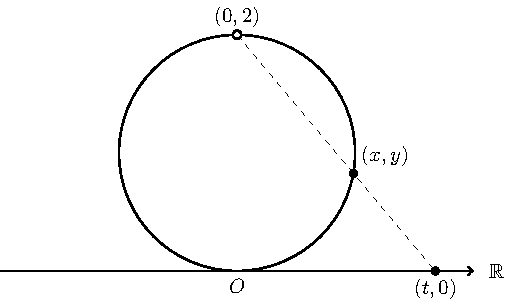
\includegraphics{images/c1.1.pdf}
    \caption{Окружность с выколотым полюсом и прямая гомеоморфны.}
    \label{fig:c1.1}
\end{figure}


\subsection{Связность}
\begin{definition}
    Топологическое пространство $X$ называется \textit{связным}, если не существует двух открытых непустых непересекающихся множеств $A$ и $B$ таких, что $X = A \cup B$.
\end{definition}

\begin{statement}
    Отрезок вещественной прямой в стандартной топологии связен.
\end{statement}
\begin{proof}
    От противного. Пусть отрезок несвязен. $\exists A, B \subset \R: \ [a, b] = A \cup B, \ A \cap B = \emptyset$, где $A, B$ — открытые множества. Пусть $\alpha \in A$, тогда $[a, \alpha) \subset A$ (т.к. A открыто). Рассмотрим $\alpha_0 = \sup\{ {\alpha}: [a, \alpha) \subset A\}$. \\
    Пусть $\alpha_0 \in A$, тогда:
    \begin{enumerate}
        \item $\alpha_0 = b \Rightarrow B = \emptyset$ — противоречие.
        \item $\alpha_0 < b \Rightarrow \alpha_0$ входит в $A$ с окрестностью $\Rightarrow$ существует $(\alpha_0 - \epsilon, \alpha_0 + \epsilon) \in A \Rightarrow \alpha_0$ — не супремум — противоречие.
    \end{enumerate}
\end{proof}

% конец первой лекции
%\begin{statement}
    Непрерывный образ связного пространства связен.
\end{statement}
\begin{proof}
    $f: X \to Y$. От противного. Пусть образ несвязен. Тогда $Im f = A \cup B$, где A, B — открытые и непустые множества, $A \cap B = \emptyset$. $f^{-1}(A)$ открыто, $f^{-1}(B)$ открыто. Если множества не пересекаются, то и их образы не пересекаются. Так как множества не пусты, то и их образы не пусты. $f^{-1}(A) \cup f^{-1}(B) = X \Rightarrow X$ не связно — противоречие. 
\end{proof}

\begin{remark}
    Связность является топологическим инвариантом.
\end{remark}


\subsection{Линейная связность}
\begin{definition}
    \textit{Непрерывная кривая (параметрическая)} — непрерывное отображение ненулевого отрезка в топологическое пространство. $\gamma: [a,b] \to X$, где $\gamma$ непрерывна.
\end{definition}

$\gamma: [0, 2 \pi] \to \R^{2}$

$\begin{cases}
    x = \cos{t}, \\
    y = \sin{t}, \\
    t \in [0, 2 \pi].
\end{cases}$

\begin{definition}
    Топологическое пространство называется \textit{линейно связным}, если любые две его точки можно соединить кривой.
\end{definition}

$x, y$ — точки $X$, тогда $\exists \gamma: [\alpha, \beta] \to X: \ \gamma(\alpha) = x, \ \gamma(\beta) = y$

\begin{statement}
    Образ линейно связного пространства линейно связен.
\end{statement}
\begin{proof}
    Композиция непрерывных отображений непрерывна:
    $$\gamma: [\alpha, \beta] \to X, \ f: X \to Y.$$
\end{proof}

\begin{statement}
    Если топологическое пространство линейно связно, то оно связно. (Наоборот, вообще говоря, неверно — как задачу можно попросить привести контрпример).
\end{statement}
\begin{proof}
    Пусть топологическое пространство линейно связно, но не связно. Тогда $X = A \cup B$. Возьмём $x \in A, \ y \in B$. Пользуемся линейной связностью: $\gamma: [0, 1] \to X$, $\gamma$ непрерывна, $\gamma(0) = A, \ \gamma(1) = B, \ Im \gamma$ в $X$ — связно.
    $Im \gamma \cap A$ — открыто в топологии образа $Im \gamma$, индуцированного топологии на $X$ (пользуемся топологией на подмножестве), $Im \gamma \cap B$ — открыто в топологии образа $Im \gamma$, индуцированного топологии на $X$ — получили противоречие с тем, что отрезок несвязен.
\end{proof}


\subsection{Компактность}
\begin{definition}
    Топологическое пространство \textit{компактно}, если из его любого открытого покрытия можно выбрать конечное подпокрытие.
\end{definition}

\begin{statement}
    Непрерывный образ компакта является компактом.
\end{statement}
\begin{proof}
    Пусть $f: X \to Y$. Покрываем образ: $Im f \subseteq \bigcup_{\alpha} U_{\alpha}$ — покрытие.
    $X \subset \bigcup_{\alpha} f^{-1}(U_{\alpha})$ — открытое покрытие $X$ (т.к. $f$ непрерывно).
    $X \subset \bigcup_{i = 1}^{n} f(U_{i})$ — конечное подпокрытие.
    Пользуемся компактностью $X$: $Im f \subset \bigcup_{i = 1}^{n} f(U_{i})$
\end{proof}

\begin{remark}
    Компактность является топологическим инвариантом.
\end{remark}

\begin{statement}
    Замкнутое подмножество компакта есть компакт.
\end{statement}
\begin{proof}
    $M \subset X \subset Y$, $M$ замкнуто, $X$ компактно, $Y$ — топологическое пространство.
    $M \subset \bigcup_{\alpha} U_{\alpha}$ открытое покрытие $M$.
    $(Y \setminus M) \cup \bigcup_{\alpha} U_{\alpha}$ — открытое покрытие.
    Выберем в нём конечное подпокрытие:
    $X \subset (Y \setminus M) \cup \bigcup_{i = 1}^n U_i$ — конечное подпокрытие.
    $M \subset \bigcup_{i = 1}^n U_i$.
\end{proof}


\subsection{Хаусдорфовость}
\begin{definition}
    Топологическое пространство $X$ называется \textit{хаусдорфовым}, если у любых двух его различных точек существуют непересекающиеся окрестности.
\end{definition}

$\tau = {X, \emptyset} \Rightarrow X$ не хаусдорфово.

\begin{lemma}
    Компакт в хаусдоровом пространстве является замкнутым множеством.
\end{lemma}
\begin{proof}
    $M \subset X$, $M$ — компакт.
    $x_0 \in X \setminus M$, $y \in M$.
    Пользуемся хаусдорфовостью: $x_0 \in U_{x_0}^y, \ y \in V_y, \ U_{x_0}^y \cap V_y = \emptyset$.
    $\bigcup_{y \in M} V_y$ — открытое покрытие всего множества $M$.
    Пользуемся компактностью: выберем конечное подпокрытие $M \subset \bigcup_{i = 1}^n v_{y_i}, \ y_i \in M$.
    $\bigcap_{i = 1}^n U_{x_0}^{y_i} = U$, $x_0 \in U$, $U \cap V_{y_i} = \emptyset$, $U$ открытое $\Rightarrow X \setminus M$ открыто.
\end{proof}

\begin{statement}
    $f: X \to Y$, $f$ — непрерывная биекция, $X$ — компакт, $Y$ — хаусдорфово топологическое пространство $\Longrightarrow$ $f$ — гомеоморфизм.
\end{statement}
\begin{proof}
    $f: X \to Y$, $X$ замкнуто, $M \subset X$, $M$ замкнуто $\Rightarrow M$ компактно $\Rightarrow f(M) \subset Y$, где $f(M)$ тоже компактно (т.к. $f$ непрерывно) $\Rightarrow f(M)$ замкнуто в $Y$. 
\end{proof}

Фактор-топология: дано топологическое пространство $X$, и на нём задано отношение эквивалентности: $f: X \to X \setminus \sim$. $f$ сопоставляет каждой точке из $X$ её класс эквивалентности.
Топология $X \setminus \sim$ задаётся отображением $f$.

Важный пример не забудь добавить.

% конец второй лекции

\end{document}